\documentclass{article}


\usepackage{arxiv}

\usepackage[utf8]{inputenc} % allow utf-8 input
\usepackage[T1]{fontenc}    % use 8-bit T1 fonts
\usepackage{hyperref}       % hyperlinks
\usepackage{url}            % simple URL typesetting
\usepackage{geometry}
\geometry{margin=0.5in}
\usepackage{multirow}
\usepackage{float}
\usepackage{graphicx}
\usepackage{caption}
\usepackage{filecontents}
\usepackage{subcaption} % Add the subcaption package
\usepackage[title]{appendix}
\usepackage{fancyhdr}
\usepackage{array}
\usepackage{booktabs}       % professional-quality tables
\usepackage{amsfonts}       % blackboard math symbols
\usepackage{nicefrac}       % compact symbols for 1/2, etc.
\usepackage{microtype}      % microtypography
\usepackage{lipsum}
\usepackage{graphicx}
\pagestyle{fancy}
\usepackage{amsmath}
\graphicspath{ {./images/} }
\usepackage[compact]{titlesec}         % you need this package
\titlespacing{\subsection}{0pt}{5pt}{0pt} % this reduces space between (sub)sections to 0pt, for example


\title{COMP 551 Assignment 2 Report - Fall 2024}


\author{
 Hathaway Hao \\
  261071268\\
  %% examples of more authors
   \And
 Yifan Lin \\
  261078741\\
  \And
 Michael Yu \\
  261070826\\
  %% \AND
  %% Coauthor \\
  %% Affiliation \\
  %% Address \\
  %% \texttt{email} \\
  %% \And
  %% Coauthor \\
  %% Affiliation \\
  %% Address \\
  %% \texttt{email} \\
  %% \And
  %% Coauthor \\
  %% Affiliation \\
  %% Address \\
  %% \texttt{email} \\
}

\begin{document}
\maketitle
\begin{abstract}
\textit {Statistical learning is key to Machine Learning, so we evaluated linear regression and logistic classification on the Infrared Thermography and CDC Diabetes datasets. We implemented analytical least squares, gradient descent, and mini-batch SGD. Our experiments analyzed performance, feature importance, and the effects of training size, mini-batch size, and learning rates. Cross-validation was used to prevent overfitting, and we compared analytical and iterative approaches for linear regression. Key findings show the importance of learning rates, batch size, and computational trade-offs. This study marks our first application of machine learning and identifies areas for future research.}

\end{abstract}



\section{Task 1: Linear Regression with Non-Linear Basis Functions}

\subsection{Introduction}
\noindent The main objective of Task 1 is to explore the effectiveness of Gaussian basis functions in approximating non-linear relationships. We aim to demonstrate how increasing the complexity of a model by adding more basis functions affects its performance, highlighting the trade-off between underfitting and overfitting. Our approach starts with generating synthetic data from a non-linear function, and then attempting to approximate this function using a linear combination of Gaussian basis functions. We then can observe how model complexity by changing the number of basis functions, which influences the quality of fit and generalization performances.


\subsection{Methodology}
\paragraph{Data Generation}
We begin by generating a synthetic dataset that represents a non-linear relationship. The true function is defined as:
\[
y(x) = \sin(\sqrt{x}) + \cos(x) + \sin(x) + \epsilon
\]

\begin{figure}[h]
    \centering
    \begin{minipage}{0.45\textwidth}
        \centering
        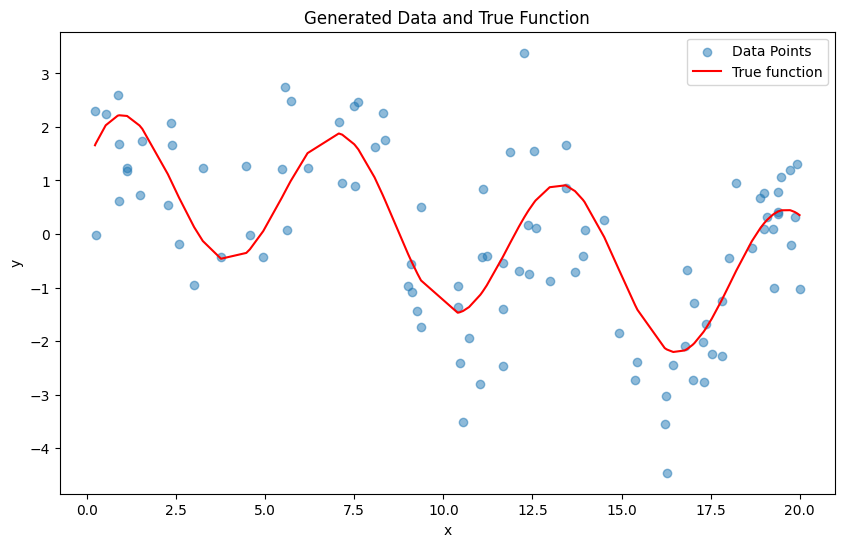
\includegraphics[width=\textwidth]{figures/data.png} 
        \caption{Non-linear data generation}
        \label{data}
    \end{minipage}\hfill
    \begin{minipage}{0.55\textwidth}
        \centering
        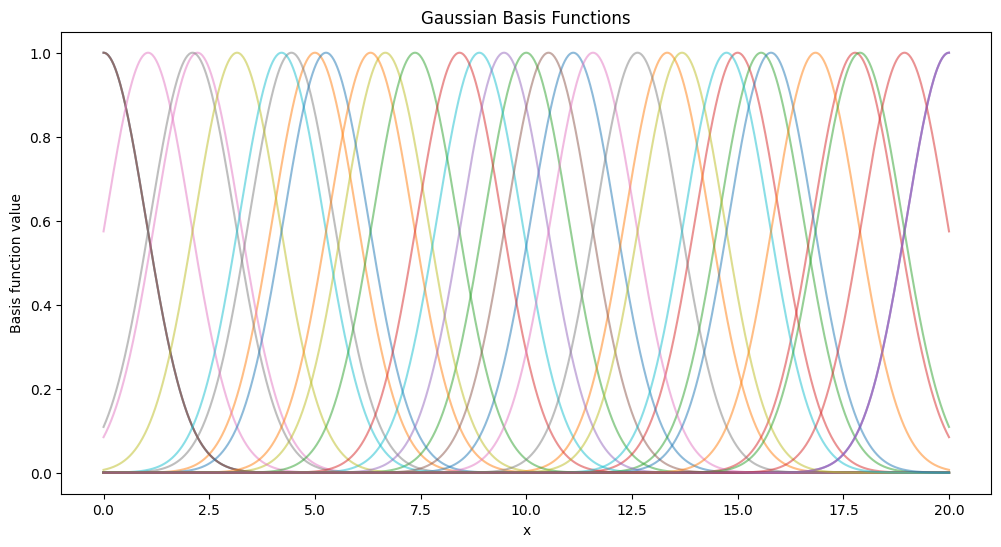
\includegraphics[width=\textwidth]{figures/gaussian_basis.png} 
        \caption{Gaussian basis for range of generated data}
        \label{gaussian}
    \end{minipage}
\end{figure}
Where $x$ is uniformly sampled from the range $[0, 20]$, and $\epsilon$ is Gaussian noise with mean 0 and variance 1. See Figure \ref{data}, the scatter plot of the generated data shows the noisy observations along with the true underlying function. The noise in the data simulates real-world measurement errors, adding complexity to the approximation task.


\paragraph{Gaussian Basis Functions}
To explore the Gaussian basis function, we transform the original input features by using Gaussian basis functions of the form:
\[
\varphi(x, \mu, \sigma) = \exp\left(-\frac{(x - \mu)^2}{2\sigma^2}\right)
\]
Where $\mu$ is the mean of the Gaussian and $\sigma$ is the standard deviation. We fix $\sigma = 1$ and vary the number of basis functions from 0 to 100, with their centers ($\mu$) evenly spaced across the input range. Shown in Figure \ref{gaussian}, demonstrates how these functions can capture local patterns in the data. Each basis function responds to inputs near its center and to distant inputs.

\paragraph{Model Fitting}
We implement a LinearRegression class that fits the model using the pseudoinverse method:
\[
w = (X^T X)^+ X^T y
\]
Here, we fit multiple models, each with a different number of basis functions (0, 10, 20, ..., 100),  visualize the fitted curves alongside the true function and the noisy data points.

\section{Task 2: Non-Linear Basis Functions}

\subsection{Introduction}
\noindent Introduction


\subsection{Methodology}
\paragraph{Methodology}


\section{Task 3: Regularization with Cross-Validation}

\subsection{Introduction}
\noindent Introduction
In this task, we implemented both \textbf{L1 (Lasso)} and \textbf{L2 (Ridge)} regularization into a linear regression model using synthetic data transformed by Gaussian basis functions. We conducted cross-validation to evaluate model performance under different values of the regularization parameter $\lambda$, ranging from $10^{-4}$ to $10^2$. Furthermore, we performed a \textbf{bias-variance decomposition} to analyze the effects of regularization on model complexity. This journal discusses each aspect of the implementation, followed by an analysis of the resulting error and bias-variance graphs.


\subsection{Methodology}
\paragraph{Implementation of L1 and L2 Regularization}
For L1 regularization (Lasso), the goal is to minimize the sum of squared residuals while also penalizing the absolute values of the weights $w$. The loss function for \textbf{L1 regularization} is given by:

$$
J(w)=\frac{1}{2 m} \sum_{i=1}^m\left(y^{(i)}-w^T x^{(i)}\right)^2+\lambda \sum_{j=1}^n\left|w_j\right|
$$


Here, the first term represents the mean squared error (MSE), and the second term is the L1 penalty on the weights. The parameter $\lambda$ controls the strength of the regularization: a larger $\lambda$ forces more weights to become zero, making the model sparser.

For \textbf{L2 regularization (Ridge)}, the penalty is applied to the squared values of the weights, resulting in the following loss function:

$$
J(w)=\frac{1}{2 m} \sum_{i=1}^m\left(y^{(i)}-w^T x^{(i)}\right)^2+\frac{\lambda}{2} \sum_{j=1}^n w_j^2
$$

In this case, the second term is the L2 penalty, which tends to shrink the weights towards zero without making them exactly zero. Again, $\lambda$ controls the regularization strength, helping reduce over-fitting by penalizing large weights.

Both these regularization methods were implemented by modifying the loss functions accordingly and using gradient descent to update the weights iterative.

\paragraph{Cross-Validation for Model Assessment}
For each $\lambda$ value, we used \textbf{10-fold cross-validation} to calculate the training and validation \textbf{MSE}. Cross-validation enabled us to assess how well the model generalized to unseen data and provided reliable estimates of the validation error for each $\lambda$. This evaluation helped us determine which $\lambda$ value minimized the validation error. The model is trained on 9 folds and tested on the remaining 1 fold, repeating this process 10 times. The MSE for the training and validation sets is computed as:

$$
\mathrm{MSE}=\frac{1}{m} \sum_{i=1}^m\left(y^{(i)}-\hat{y}^{(i)}\right)^2
$$

where $y^{(i)}$ represents the true value and $\hat{y}^{(i)}$ is the predicted value. By averaging the MSE across all folds, we obtained a reliable estimate of the model's generalization performance.

\paragraph{Bias-Variance Decomposition}
To analyze the bias-variance trade-off, we decomposed the total error into three components: bias, variance, and noise variance. The bias squared is calculated as:

$$
\operatorname{Bias}^2=\frac{1}{m} \sum_{i=1}^m\left(\mathbb{E}\left[\hat{y}^{(i)}\right]-y^{(i)}\right)^2
$$


Here, $\mathbb{E}\left[\hat{y}^{(i)}\right]$ is the expected prediction over multiple datasets, and $y^{(i)}$ is the true output.

The variance measures the variability of the model's predictions across different datasets:

$$
\text { Variance }=\frac{1}{m} \sum_{i=1}^m \mathbb{E}\left[\left(\hat{y}^{(i)}-\mathbb{E}\left[\hat{y}^{(i)}\right]\right)^2\right]
$$


Finally, the total error combines the bias, variance, and noise variance:

$$
\text { Total Error }=\text { Bias }^2+\text { Variance }+\sigma_{\text {noise }}^2
$$

where $\sigma_{\text {noise }}^2$ represents the inherent noise in the data.

\begin{itemize}
    \item \textbf{L2 regularization} \\
    As $\lambda$ increased, the bias increased, and the variance decreased. This is expected because larger $\lambda$ values restrict model flexibility, leading to simpler models with higher bias and lower variance. The total error (bias² + variance + noise variance) increased as the model became overly simplistic at high $\lambda$ values.

    \item \textbf{L1 regularization} \\
    A similar trend was observed. As $\lambda$ increased, the bias also increased while variance decreased. However, the variance remained more stable compared to L2 regularization, suggesting that L1 regularization helped retain some model flexibility even at larger $\lambda$ values.
\end{itemize}

\paragraph{Selection of Optimal $\lambda$}
Based on the validation error plots, the optimal $\lambda$ for both regularization methods was selected where the validation error was minimized. For L2 regularization, the optimal $\lambda$ value lay in the middle of the range (around $\lambda \approx 10$ ), where the model achieved a balance between under-fitting and over-fitting. Similarly, for L1 regularization, the optimal $\lambda$ value was also around $\lambda \approx 10$, where the validation error curve flattened.

The bias-variance decomposition further supported these choices. At the optimal $\lambda$ values, both the bias and variance were balanced, and the total error was minimized.

\subsection{Conclusion}
\begin{figure}[h]
    \centering
    \begin{minipage}{0.50\textwidth}
        \centering
        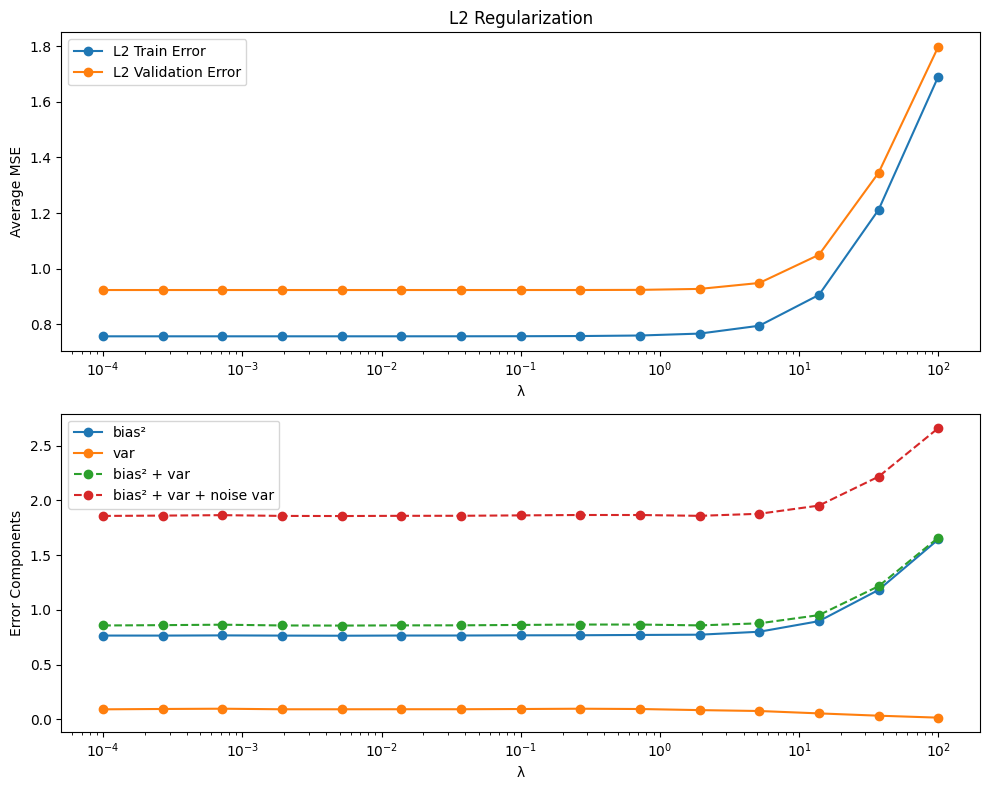
\includegraphics[width=\textwidth]{figures/L2_Regularization.png} 
        \caption{L2 Regularization}
        \label{data}
    \end{minipage}\hfill
    \begin{minipage}{0.50\textwidth}
        \centering
        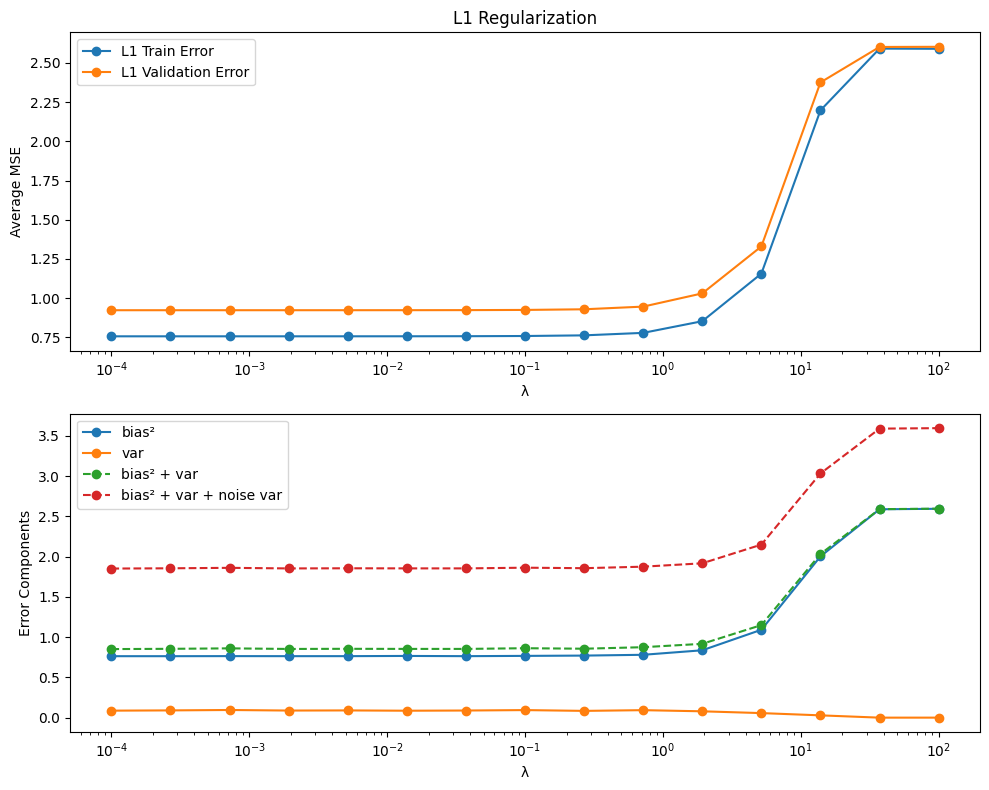
\includegraphics[width=\textwidth]{figures/L1_Regularization.png} 
        \caption{L1 Regularization}
        \label{gaussian}
    \end{minipage}
\end{figure}

By plotting the training and validation errors as a function of $\lambda$, we observed that:\\

$\bullet$ For small $\lambda$, both L1 and L2 regularization resulted in low training errors but higher validation errors, indicating over-fitting.\\
$\bullet$ As $\lambda$ increased, the training error rose, and the validation error initially decreased before rising again at very large $\lambda$, indicating under-fitting.
\\

The bias-variance decomposition further confirmed this, showing that:\\
$\bullet$ For small $\lambda$, variance was high, while bias was low, leading to over-fitting.\\
$\bullet$ As $\lambda$ increased, the bias increased while the variance decreased, balancing the two components and minimizing the total error at an intermediate value of $\lambda$.

The optimal $\lambda$ was chosen where the validation error and total error were minimized, balancing both bias and variance effectively.

In conclusion, the implementation of L1 and L2 regularization successfully controlled the complexity of the model, helping reduce over-fitting for small $\lambda$ values and under-fitting for large $\lambda$ values. Cross-validation provided a reliable way to assess the model's performance and choose the optimal $\lambda$ for both regularization types. The\textbf{ train-validation error plots} 
and \textbf{bias-variance decomposition} illustrated the impact of regularization on model performance.

\begin{itemize}
    \item \textbf{L2 regularization} led to higher bias and lower variance as $\lambda$ increased, making the model less flexible but more stable.

    \item \textbf{L1 regularization} promoted sparsity in the model weights and maintained a more stable variance as $\lambda$ increased.
\end{itemize}

The graphs clearly demonstrated how regularization influences the bias-variance trade-off, and selecting an appropriate $\lambda$ helps achieve a balance that minimizes total error. Ultimately, both L1 and L2 regularization were effective at improving model generalization, with slightly different characteristics depending on the type of regularization.


\section{Discussion and Conclusion}



\section{Statement of Contributions}

All members contributed equally to this project. We each completed the lab independently and then combined our individual work and code to produce the final report.

\newpage
\bibliographystyle{unsrt}  
%\bibliography{references}  %%% Remove comment to use the external .bib file (using bibtex).
%%% and comment out the ``thebibliography'' section.

%%% Comment out this section when you \bibliography{references} is enabled.
\begin{thebibliography}{1}

\bibitem{Infrared Thermography Temperature} Infrared Thermography Temperature
Wang et al., 2021
https://api.semanticscholar.org/CorpusID:245585208
\label{ref:dataset1}

\bibitem{CDC Diabetes Health Indicators} CDC Diabetes Health Indicators. 2021. https://archive.ics.uci.edu/dataset/891/cdc+diabetes+health+indicators \label{ref:dataset2}

\bibitem{statistical learning} Hastie, Trevor, et al. The elements of statistical learning: data mining, inference, and prediction. Vol. 2. New York: springer, 2009. \label{statistical learning}

\bibitem{Lecture notes} Prémont-Schwarz, I. (2023). Gradient Descent. COMP 551, McGill University.\label{ref:lectures}

\bibitem{validation} James, Gareth. "An introduction to statistical learning." (2013) \label{ref:validation}

\end{thebibliography}

\begin{appendices}

\section{Default Model Parameters} \label{app:default-parameters}

\begin{table}[H]
    \centering
    \vspace{7pt} % Adjust the value as needed to control the amount of space
    \renewcommand{\arraystretch}{1.5}
    \begin{tabular}{|c|c|c|c|c|c|}
        \hline
        Model  & Max iteration & Batch Size & Learning Rate & Epsilon & Regularization Term \\
        \hline
        Linear Regression with SGD & 1500 & 16 & 1e-2 & 1e-5 & 0 \\
        Logistic Regression & 2000 & 16 & 1e-3 & 1e-7 & 0.1 \\
        \hline
    \end{tabular}
\end{table}

\section{Experiment 3}

\subsection{Training Loss History of Linear Regression with data size} \label{app:loss-history-sgd}

\begin{table}[h]
    \centering
    \begin{minipage}{0.45\textwidth}  % Adjust the width as needed
        \centering
        \begin{tabular}{|c|c|}
            \hline
            \textbf{Training Size (Proportion)} & \textbf{MSE Loss} \\
            \hline
            0.2  & 233.8436 \\
            0.3  & 100.6199 \\
            0.4  & 162.3182 \\
            0.5  & 11.3937  \\
            0.6  & 7.1098   \\
            0.7  & 0.0650   \\
            0.8  & 0.0635   \\
            \hline
        \end{tabular}
        \vspace{7pt}
        \caption{Linear in Different Training Set Sizes}
        \label{linear train size}
    \end{minipage}
    \hfill
    \begin{minipage}{0.45\textwidth}  % Adjust the width as needed
        \centering
        \begin{tabular}{|c|c|}
            \hline
            \textbf{Training Size (Proportion)} & \textbf{MSE Loss} \\
            \hline
            0.2  & 0.3201 \\
            0.3  & 0.3198 \\
            0.4  & 0.3195 \\
            0.5  & 0.3213  \\
            0.6  & 0.3191   \\
            0.7  & 0.3189   \\
            0.8  & 0.3198   \\
            \hline
        \end{tabular}
        \vspace{7pt}
        \caption{Logistic in Different Training Set Sizes}
        \label{logistic train size}
    \end{minipage}
\end{table}

\subsection{Final Loss, Mean Loss and Min Loss in Linear Regression model with different mini-batch SGD} \label{app:loss-history-sgd-log}
\begin{table}[h!]
    \centering
    \begin{tabular}{|c|c|c|c|}
        \hline
        \textbf{Batch Size} & \textbf{Final Loss} & \textbf{Mean Loss} & \textbf{Min Loss} \\
        \hline
        8   & 55391.013203 & 28565.609963 & 52.265444  \\
        16  & 2085.653474  & 149.216125   & 3.461185   \\
        32  & 0.101154     & 67.321424    & 0.086003   \\
        64  & 0.083188     & 65.046168    & 0.080201   \\
        128 & 0.068877     & 64.398326    & 0.068812   \\
        814 & 0.068739     & 63.514423    & 0.068739   \\
        \hline
    \end{tabular}
    \vspace{7pt}
    \caption{Summary of Mini-batch Size Influence on SGD Linear Regression Loss}
    \label{tab:sgd_loss}
\end{table}


\end{appendices}

\end{document}

